\section{\MakeUppercase{Порівняльний аналіз результатів}}
\label{sec:chapter3}

\subsection{Відтворення текстового аналізу}
\label{sec:text_mining}

Для відтворення текстового аналізу VOSViewer засобами Python було реалізовано алгоритм, описаний у підрозділі~\ref{sec:python_system}: токенізація абстрактів та заголовків, бінарний підрахунок термінів, фільтрація за порогом $\geq$100, застосування тезаурусу для об'єднання синонімів та морфологічних варіантів.

Порівняння частот входжень 28 ключових слів показало високу кореляцію між результатами VOSViewer та Python: коефіцієнт Пірсона $r = 0{,}923$ ($p < 0{,}001$). Відмінності в абсолютних значеннях пояснюються тим, що VOSViewer аналізував 1000 записів (файл \texttt{savedrecs.txt}), тоді як Python --- 1998 записів (\texttt{merged\_data.txt}), а також можливими розбіжностями в алгоритмах токенізації та обробки n-грам (наприклад, <<higher education>> як один термін).

Критичним фактором підвищення кореляції стало розширення тезаурусу: додавання морфологічних варіантів (skills$\to$skill, teaching$\to$teacher, students$\to$student, training$\to$training тощо) підвищило коефіцієнт кореляції з $r = 0{,}90$ до $r = 0{,}923$.

\subsection{Порівняння ко-входжень та Total Link Strength}
\label{sec:cooccurrence}

Матрицю ко-входжень побудовано для 28 ключових слів: елемент $c_{ij}$ дорівнює кількості документів, у яких одночасно зустрічаються терміни $i$ та $j$. Повна матриця наведена в Додатку~А. Мережа виявилась майже повністю зв'язною: 378 із 378 можливих пар мають ненульові ко-входження, що характерно для семантично однорідного дослідницького поля.

Total Link Strength (TLS) --- сума ко-входжень терміна з усіма іншими термінами --- є ключовою мережевою метрикою VOSViewer. Порівняння значень TLS показало високу кореляцію: $r = 0{,}919$ ($p < 0{,}001$). Різниця в абсолютних значеннях (Python-значення систематично нижчі) пояснюється різним обсягом вибірок, але ранговий порядок термінів за TLS зберігається: \textit{vet}, \textit{study}, \textit{student}, \textit{training}, \textit{teacher} --- п'ять найцентральніших термінів в обох аналізах.

\subsection{Порівняння кластеризації}
\label{sec:clustering}

Для кластеризації мережі ключових слів у Python використано алгоритм Лувена~\cite{Blondel2008}, що максимізує модулярність мережі~\cite{Newman2006}, з перебором параметра resolution від 0,5 до 2,0 з кроком 0,1. Оптимальна кількість кластерів оцінювалась за метриками ARI (Adjusted Rand Index)~\cite{Hubert1985} та NMI (Normalized Mutual Information) порівняно з 4-кластерним розбиттям VOSViewer.

Результати показали, що найкращу відповідність забезпечує розбиття на 3 кластери (ARI\,=\,0,47; NMI\,=\,0,61). При спробі отримати 4 кластери метрики знижуються (ARI\,=\,0,30--0,35), що пояснюється злиттям кластерів~3 (Педагогічна практика) та 4 (Когнітивні результати) VOSViewer в один кластер Python. Це зумовлено майже повною зв'язністю мережі (378/378 пар), що ускладнює виявлення тонких структурних відмінностей алгоритмом Лувена.

Порівняння кластерної належності (рис.~\ref{fig:cluster_comparison}) демонструє, що:
\begin{itemize}
    \item Кластер~1 (Системи та політика ПТО) відтворюється найточніше: 9 з 11 термінів збігаються.
    \item Кластер~2 (Результати навчання) також відтворюється добре: 7 з 8 термінів збігаються. Термін \textit{vet} у Python потрапляє до цього кластера замість кластера~1.
    \item Кластери~3 і 4 VOSViewer об'єднуються в один кластер Python, що включає всі 9 термінів (6 з кластера~3 та 3 з кластера~4).
\end{itemize}

\begin{figure}[htbp]
    \centering
    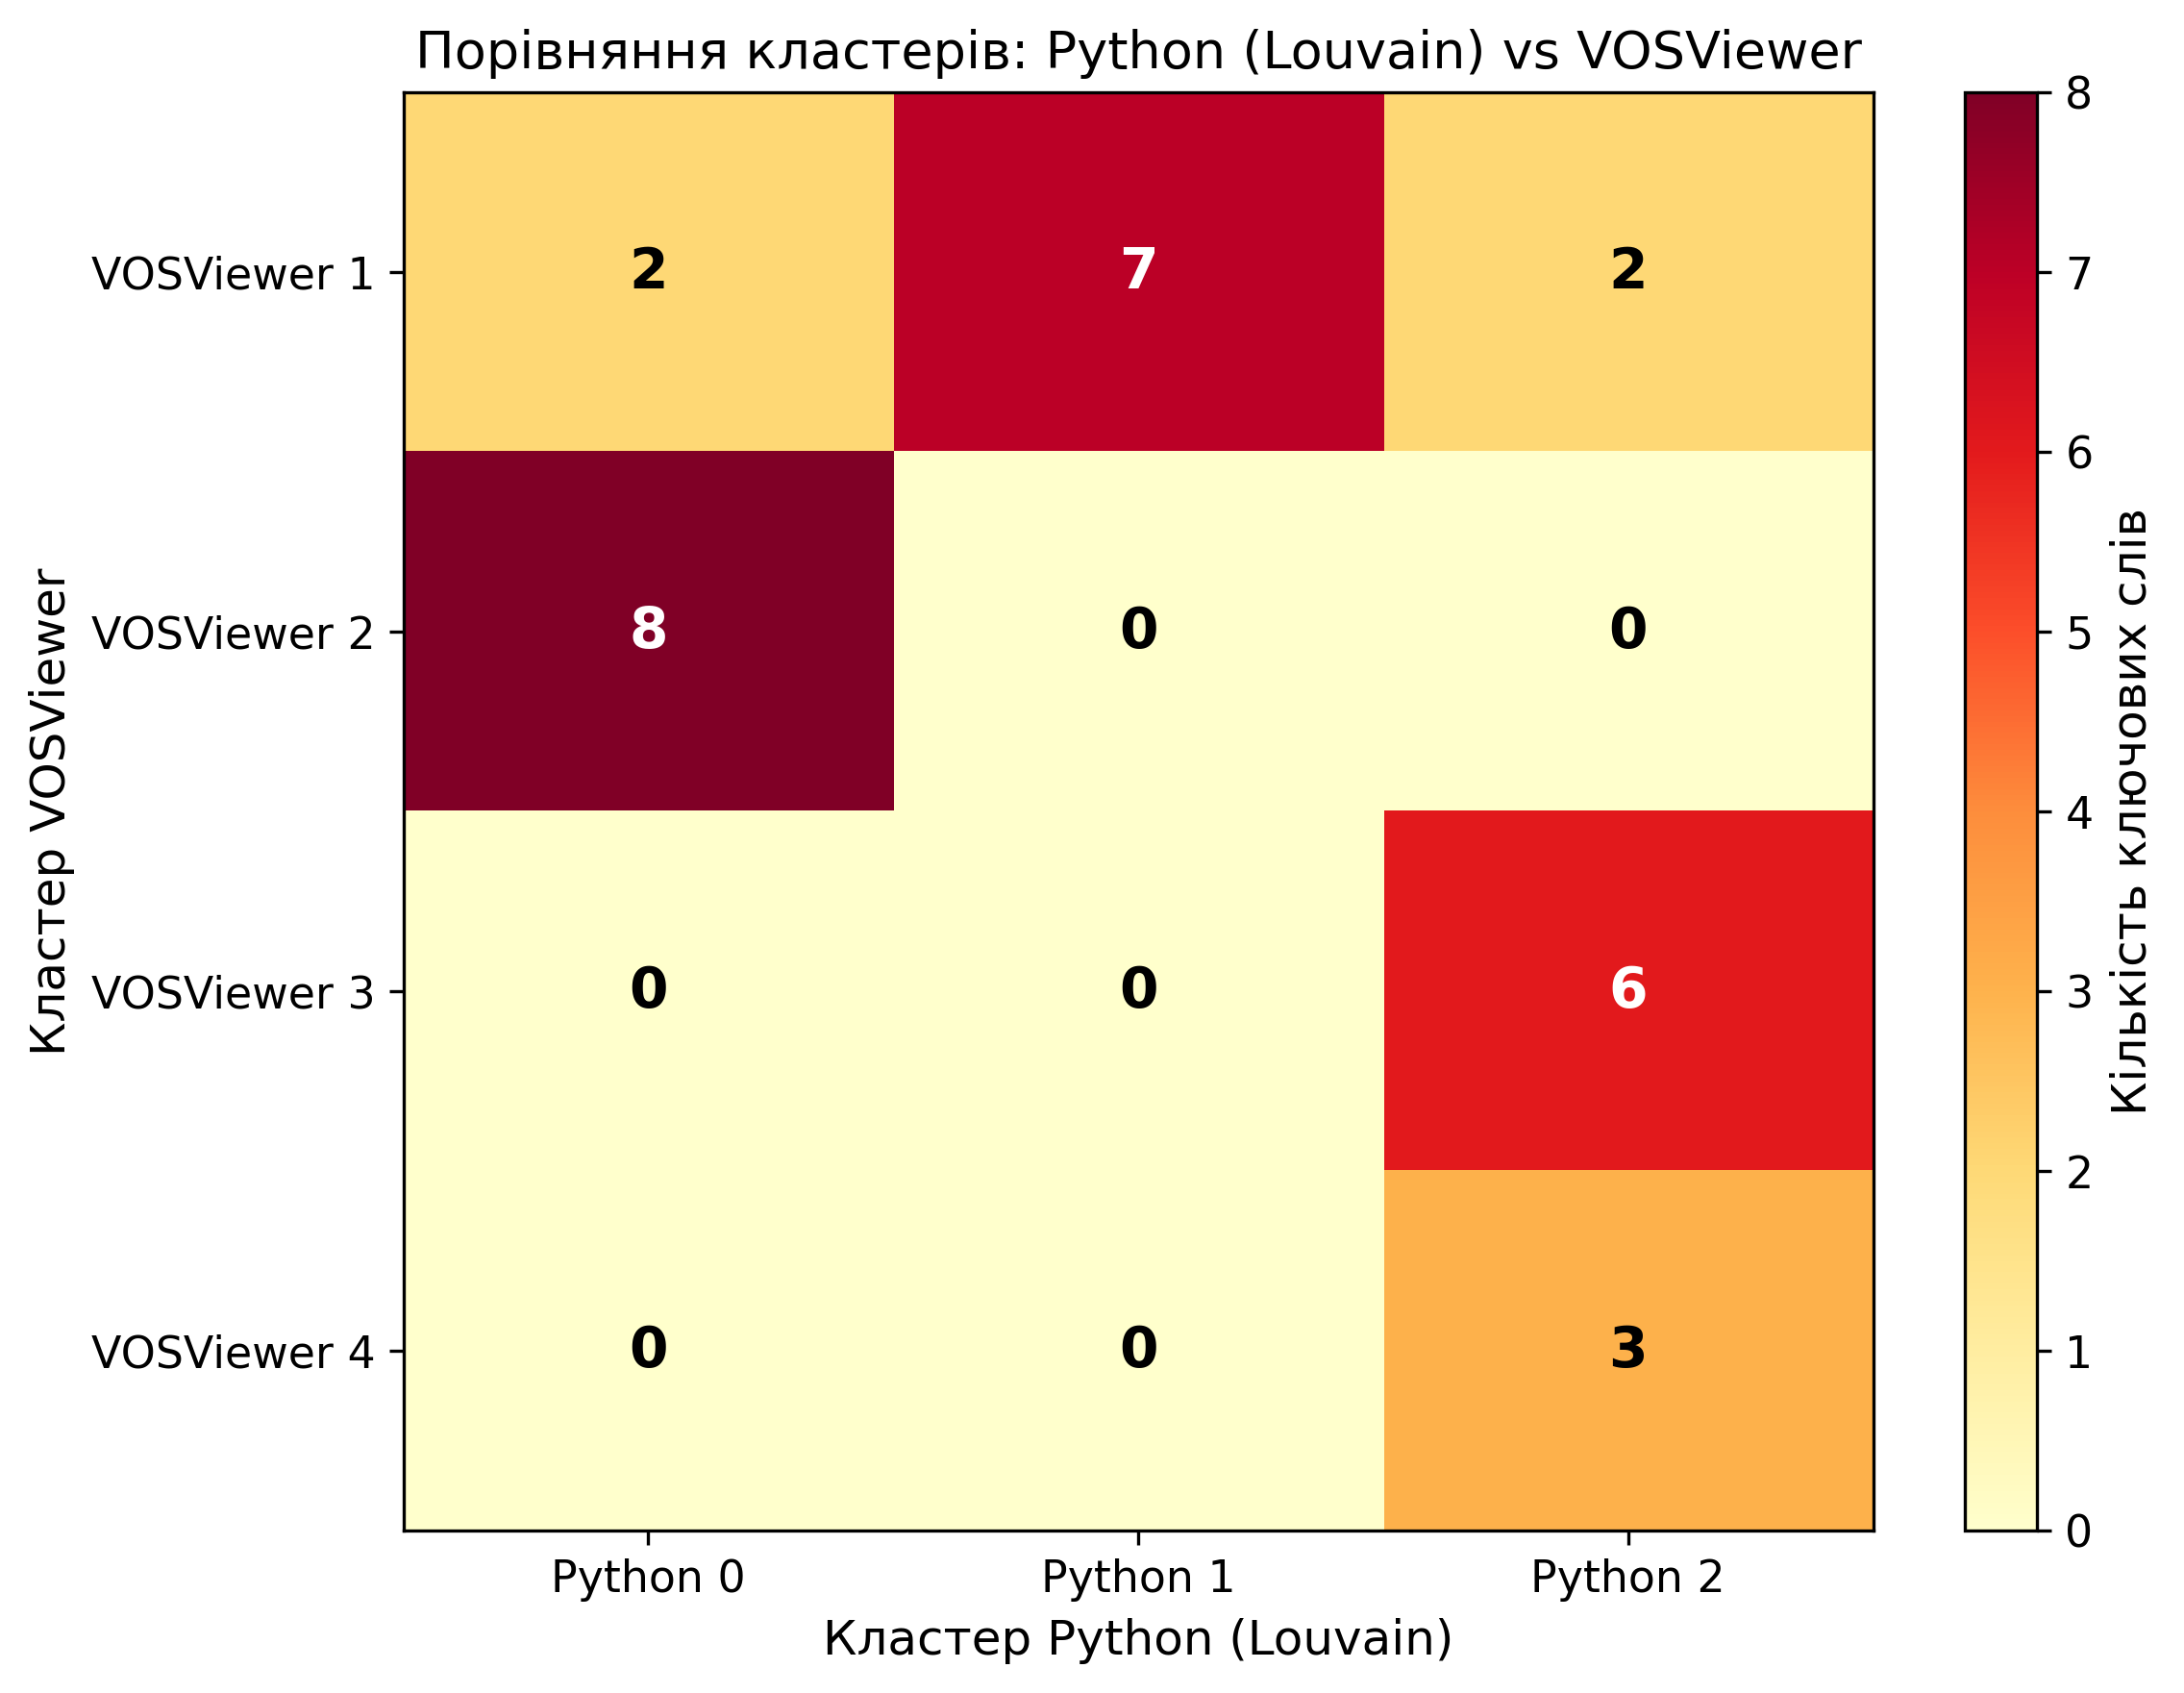
\includegraphics[width=\linewidth]{media/fig_cluster_comparison.png}
    \caption{Порівняння кластерів Python та VOSViewer.}
    \label{fig:cluster_comparison}
\end{figure}

\subsection{Порівняння мережевих візуалізацій}
\label{sec:network_comparison}

Мережу ключових слів побудовано в Python за допомогою бібліотеки NetworkX~\cite{Hagberg2008} із використанням алгоритму spring layout (Fruchterman--Reingold) для автоматичного розташування вузлів (рис.~\ref{fig:network_python}).

\begin{figure}[htbp]
    \centering
    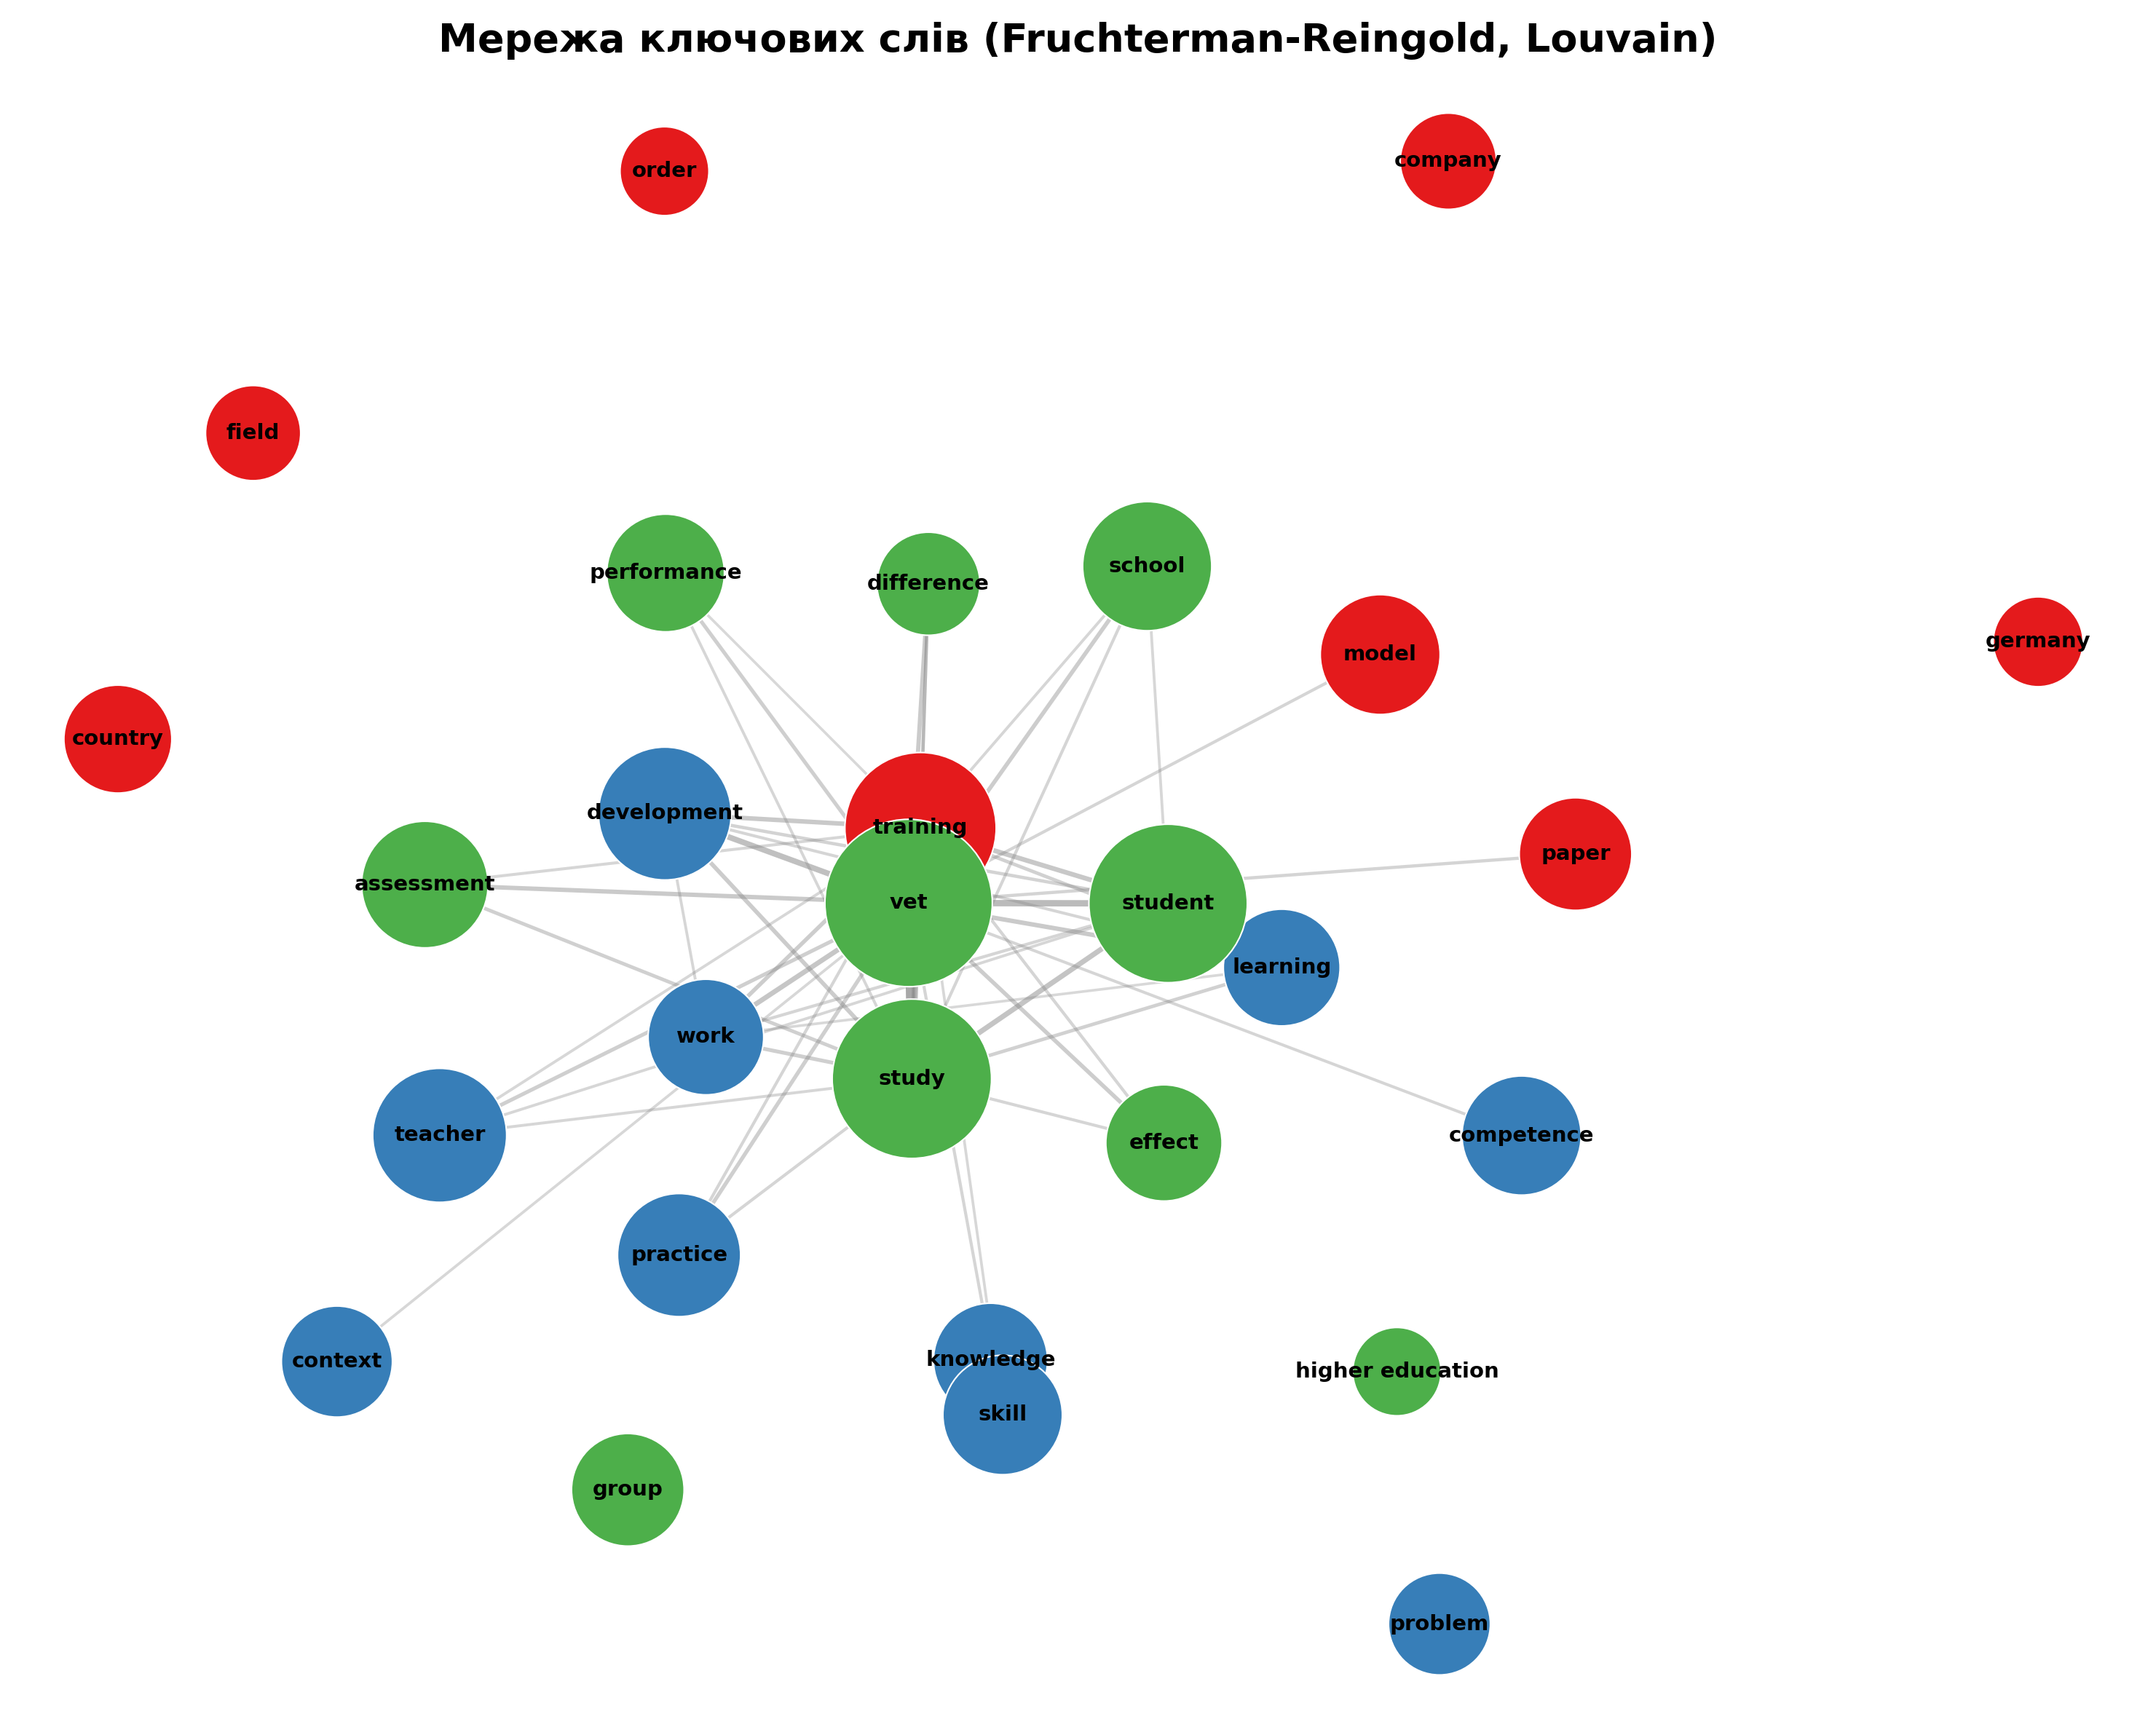
\includegraphics[width=\linewidth]{media/fig_network_python.png}
    \caption{Мережа ключових слів, побудована засобами Python (spring layout).}
    \label{fig:network_python}
\end{figure}

Порівняння мережевих візуалізацій <<пліч-о-пліч>> (рис.~\ref{fig:network_comparison}) показує, що загальна топологія мережі зберігається: центральне положення термінів \textit{vet}, \textit{training}, \textit{student}, \textit{study}; периферійне розташування термінів \textit{germany}, \textit{order}, \textit{company}. Відмінності полягають у точному просторовому розташуванні вузлів, що зумовлено різними алгоритмами (VOS у VOSViewer vs.\ Fruchterman--Reingold у NetworkX).

\begin{figure}[htbp]
    \centering
    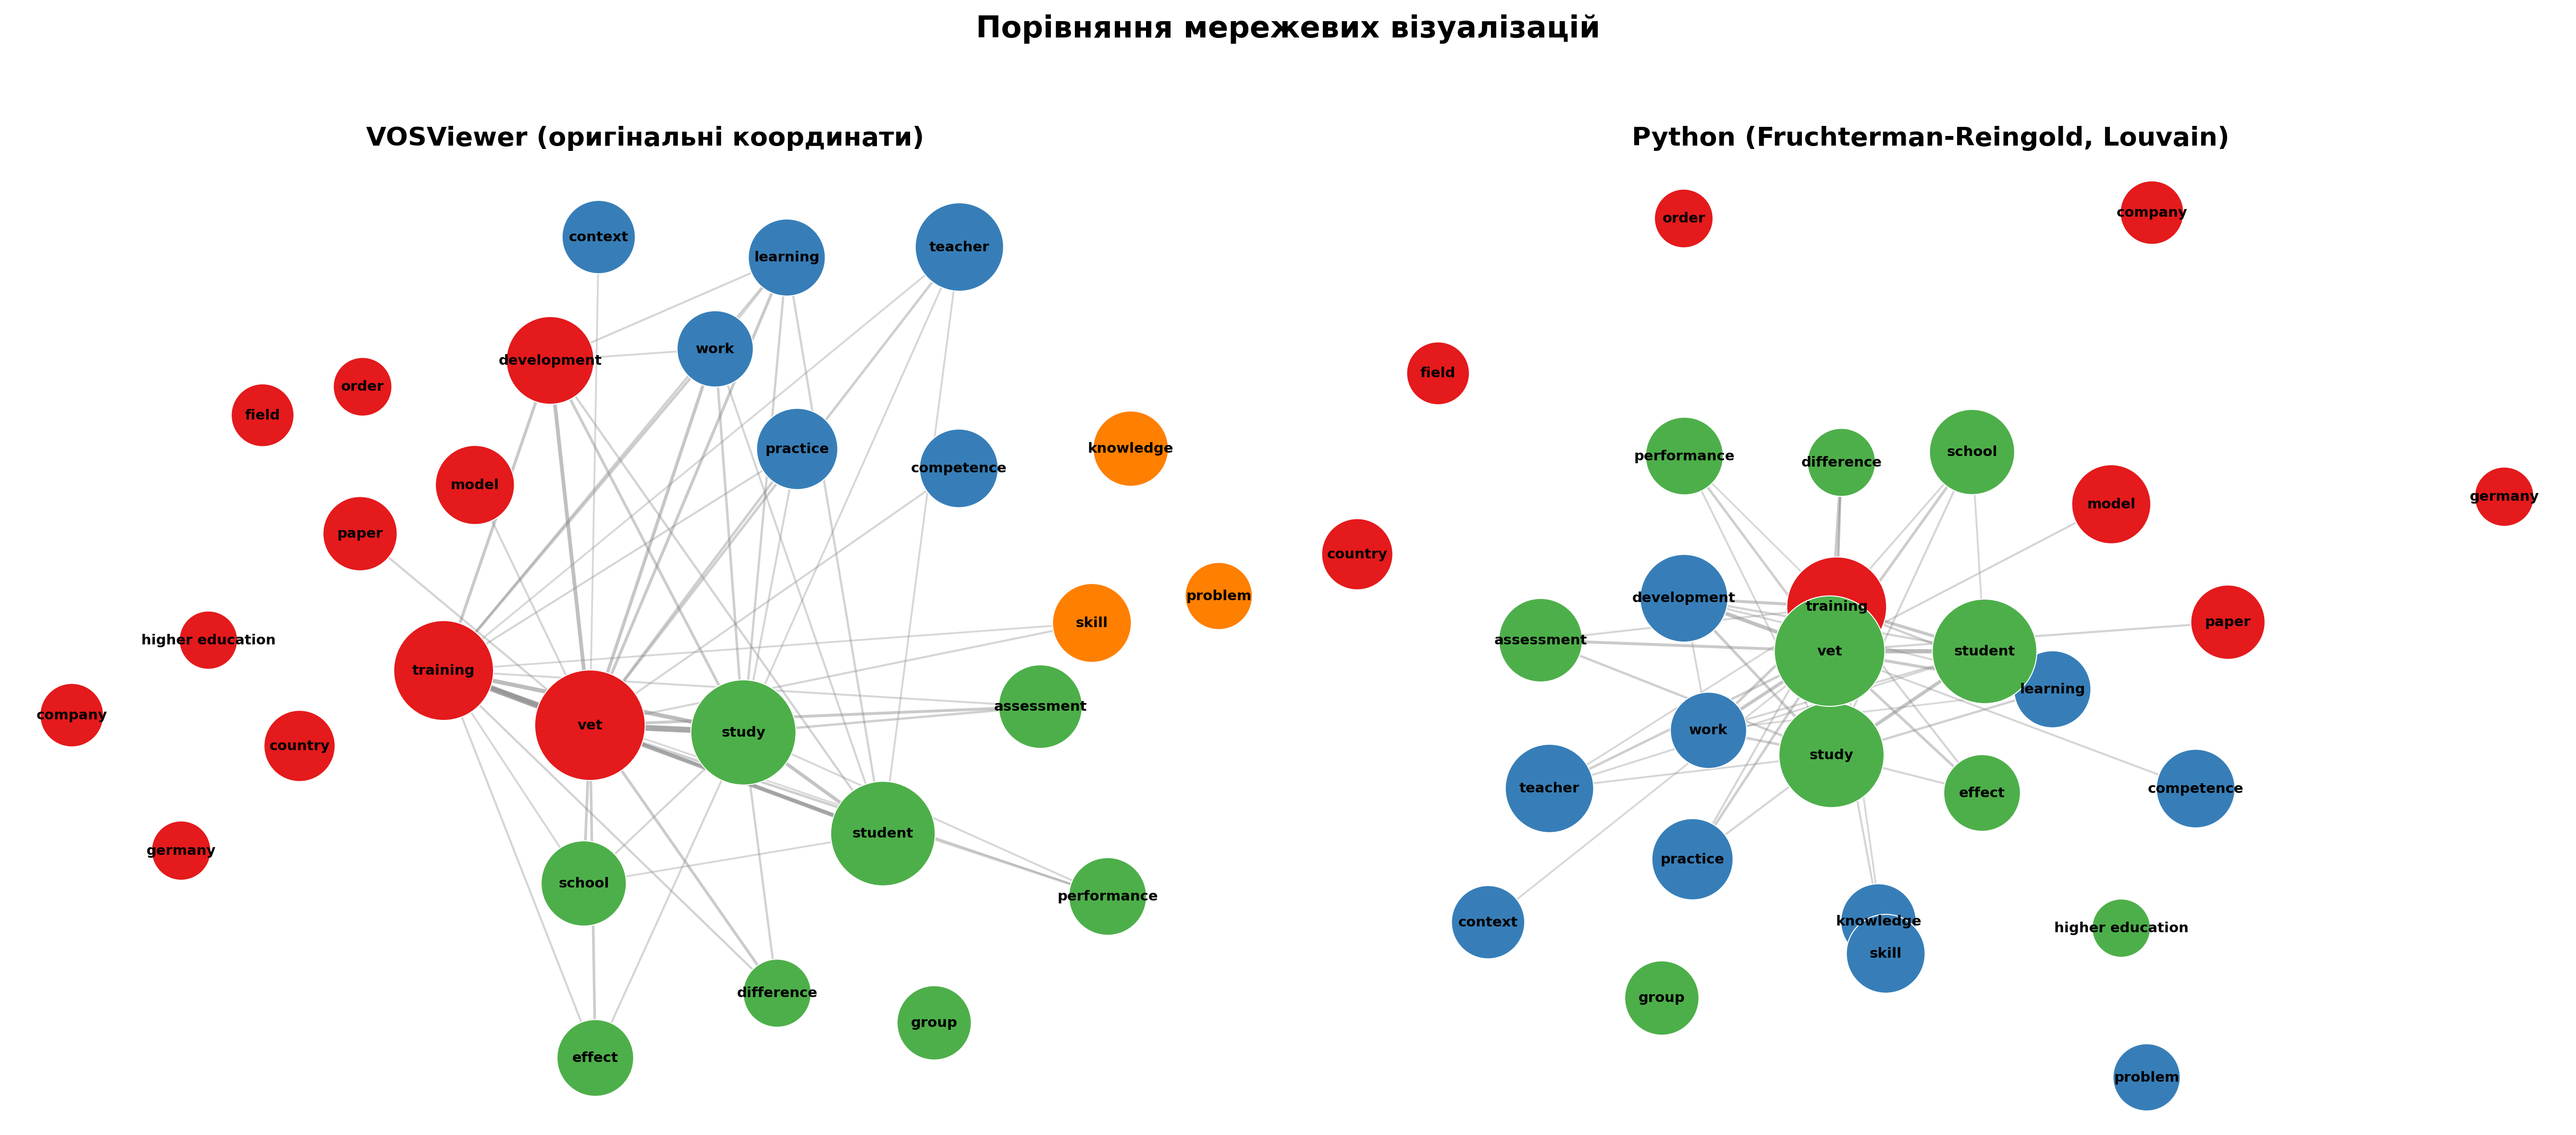
\includegraphics[width=\linewidth]{media/fig_network_comparison.png}
    \caption{Порівняння мережевих візуалізацій VOSViewer та Python.}
    \label{fig:network_comparison}
\end{figure}

Накладна карта нормалізованої цитованості (рис.~\ref{fig:overlay_norm_citations}) дозволяє оцінити відносний науковий вплив термінів з урахуванням року публікації. Порівняння з відповідною картою VOSViewer показало кореляцію $r = 0{,}79$.

\begin{figure}[htbp]
    \centering
    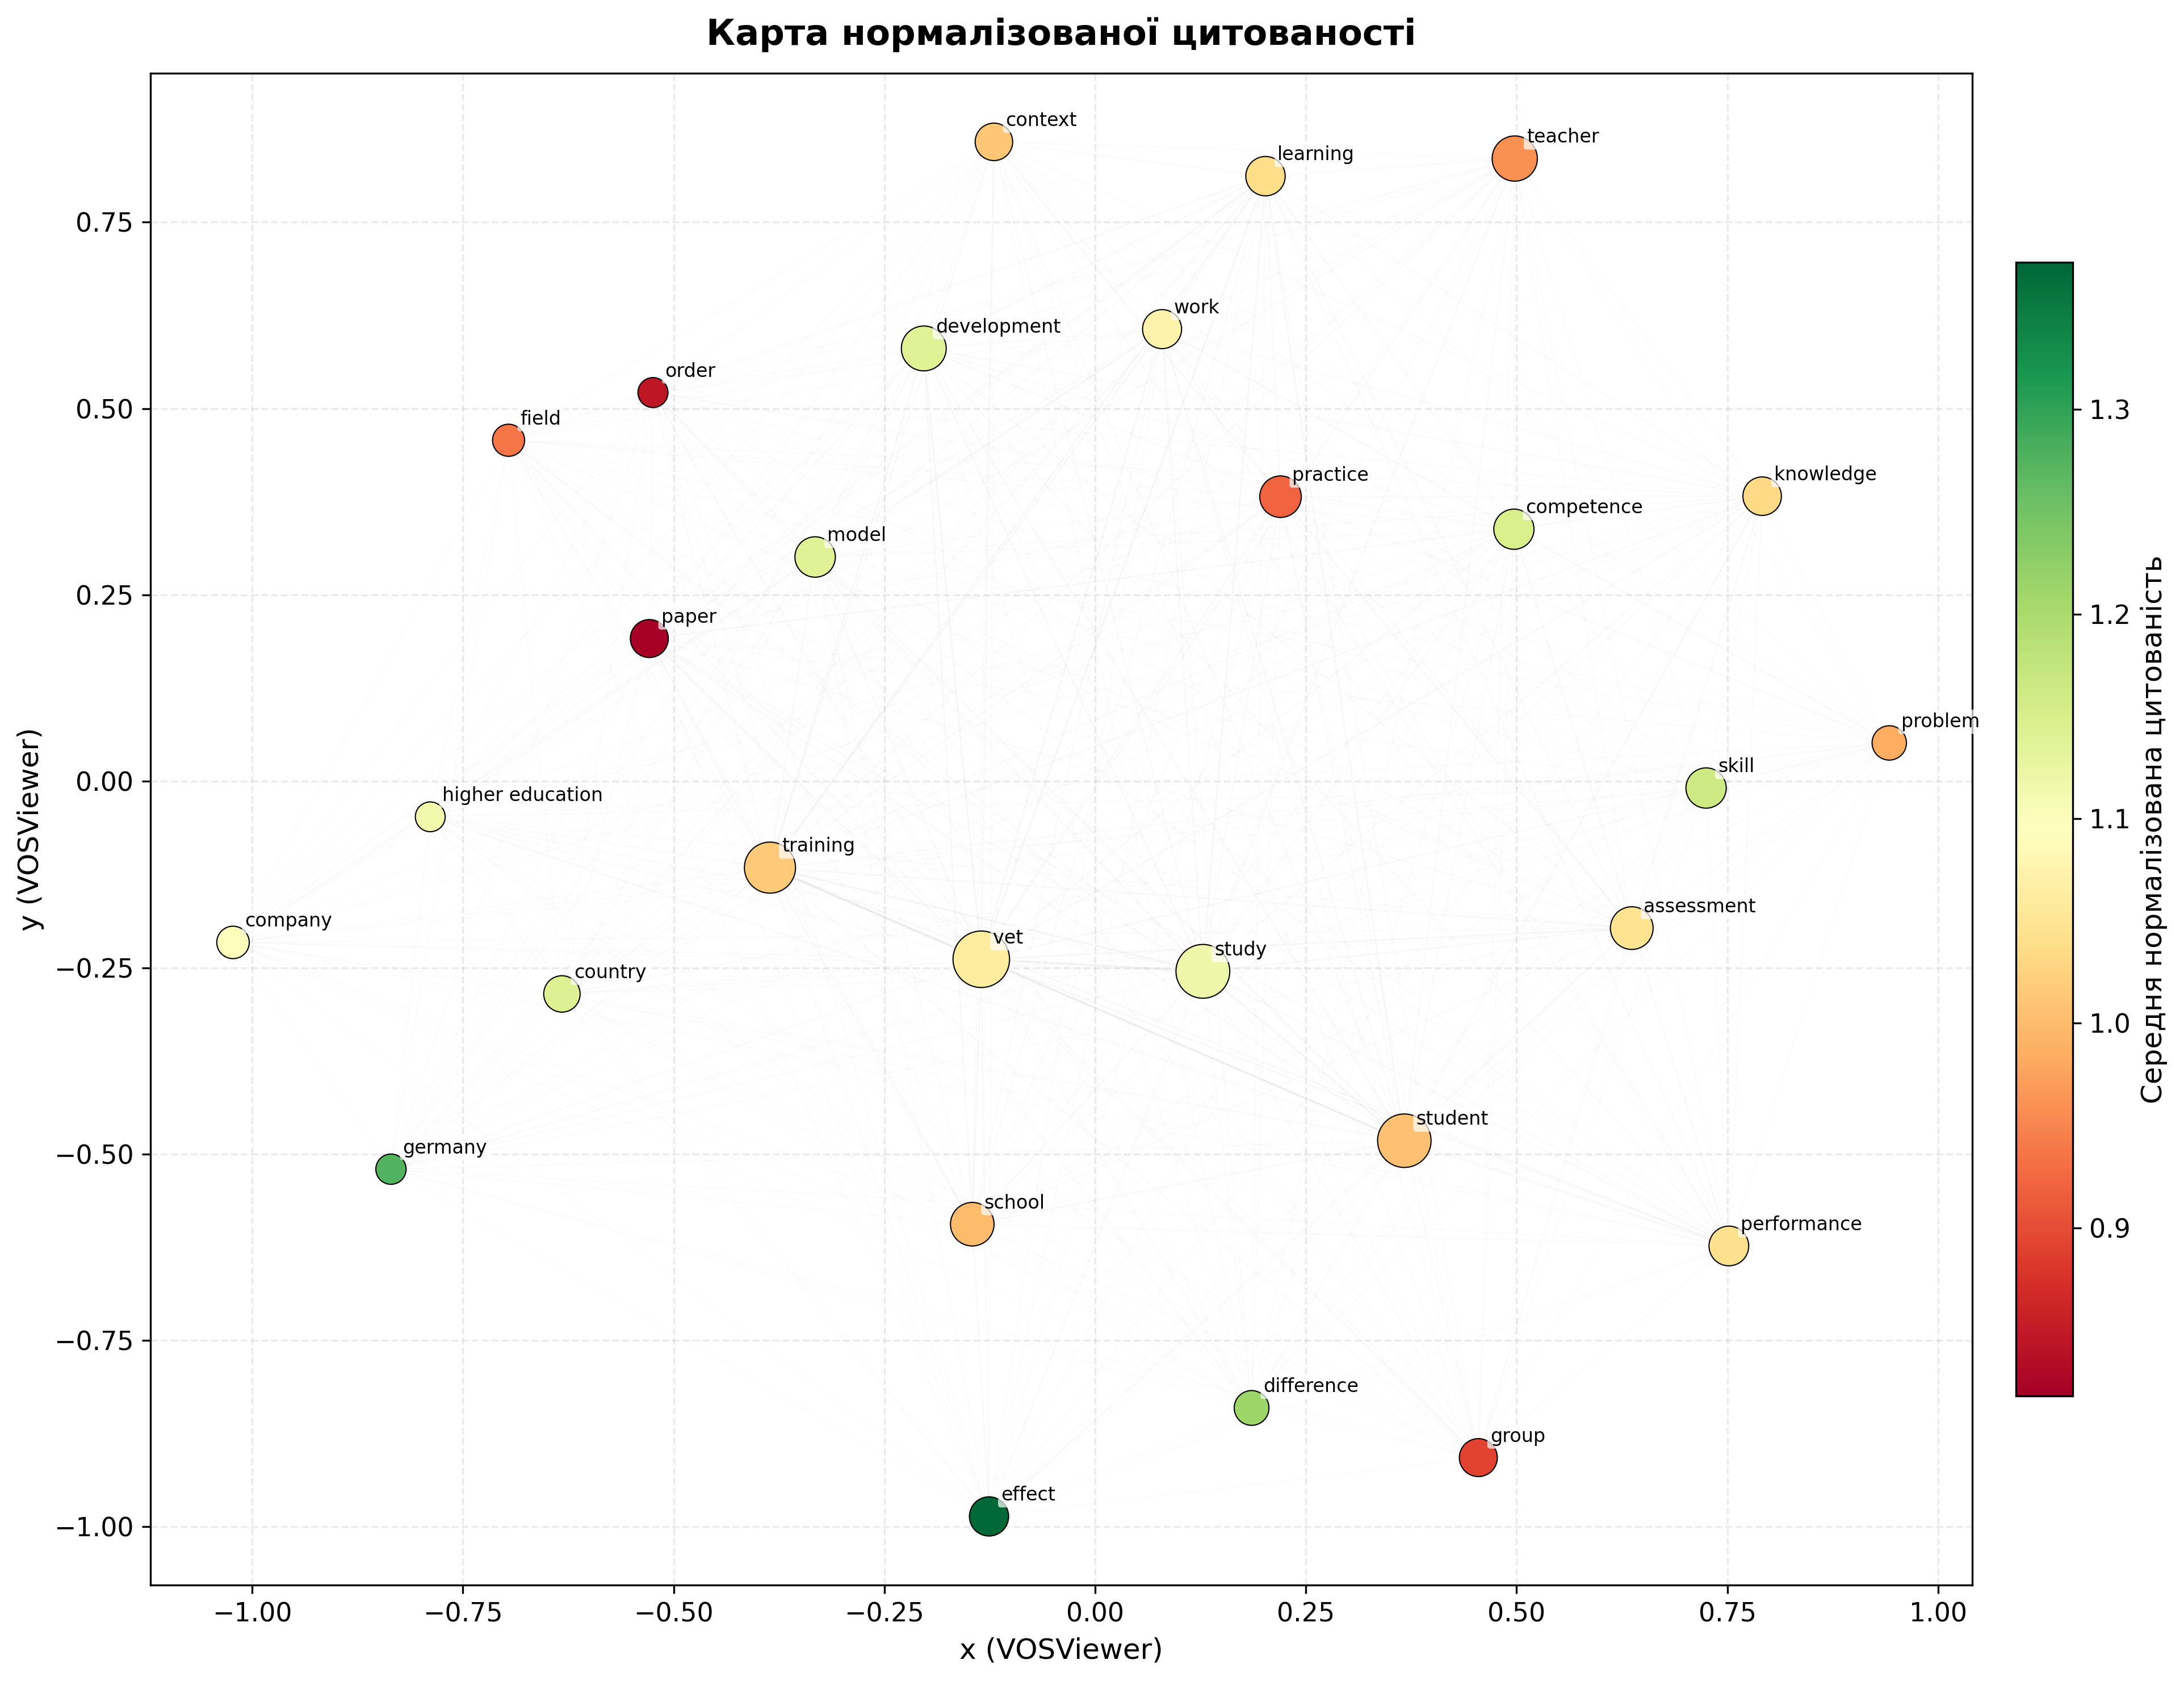
\includegraphics[width=\linewidth]{media/fig_overlay_norm_citations.png}
    \caption{Карта нормалізованої цитованості ключових слів (Python).}
    \label{fig:overlay_norm_citations}
\end{figure}

\subsection{Підсумок порівняння}
\label{sec:comparison_summary}

Зведені результати порівняння метрик VOSViewer та Python для всіх 28 ключових слів наведено в табл.~\ref{tab:comparison}.

\begin{table}[htbp]
\centering
\caption{Порівняння метрик VOSViewer та Python.}
\label{tab:comparison}
\scriptsize
% \caption{Порівняння метрик VOSViewer та Python}
% \label{tab:comparison}
\begin{tabular}{l|cc|rr|rr|rr|rr|rr}
\hline
Ключове слово & \multicolumn{2}{c|}{Кластер} & \multicolumn{2}{c|}{Входження} & \multicolumn{2}{c|}{TLS} & \multicolumn{2}{c|}{Сер. рік} & \multicolumn{2}{c|}{Сер. цит.} & \multicolumn{2}{c}{Сер. норм. цит.} \\
 & VOS & Py & VOS & Py & VOS & Py & VOS & Py & VOS & Py & VOS & Py \\
\hline
assessment & 2 & 2 & 473 & 339 & 6216 & 2768 & 2016.4 & 2017.0 & 13.8 & 12.8 & 1.05 & 1.05 \\
company & 1 & 1 & 158 & 81 & 2334 & 762 & 2019.9 & 2018.6 & 7.6 & 8.4 & 1.10 & 1.05 \\
competence & 3 & 0 & 371 & 224 & 6352 & 2173 & 2016.9 & 2017.5 & 17.0 & 12.6 & 1.15 & 1.05 \\
context & 3 & 0 & 280 & 206 & 4437 & 1929 & 2019.1 & 2018.8 & 8.9 & 8.1 & 1.01 & 0.95 \\
country & 1 & 1 & 250 & 153 & 3049 & 1294 & 2016.4 & 2017.6 & 14.4 & 12.3 & 1.14 & 1.10 \\
development & 1 & 0 & 574 & 443 & 8461 & 3784 & 2018.2 & 2017.4 & 12.2 & 11.4 & 1.14 & 1.01 \\
difference & 2 & 2 & 208 & 324 & 2956 & 2764 & 2016.9 & 2017.6 & 15.8 & 12.1 & 1.21 & 1.10 \\
effect & 2 & 2 & 336 & 311 & 3881 & 2564 & 2017.6 & 2017.5 & 15.9 & 11.7 & 1.37 & 1.09 \\
field & 1 & 1 & 151 & 119 & 2230 & 1075 & 2018.1 & 2017.4 & 10.2 & 11.3 & 0.94 & 1.02 \\
germany & 1 & 1 & 120 & 80 & 1769 & 669 & 2017.7 & 2017.3 & 16.3 & 16.3 & 1.28 & 1.31 \\
group & 2 & 2 & 296 & 186 & 3696 & 1522 & 2016.6 & 2016.8 & 10.7 & 10.8 & 0.89 & 0.93 \\
higher education & 1 & 0 & 112 & 85 & 1510 & 764 & 2018.7 & 2018.3 & 13.3 & 10.2 & 1.11 & 0.93 \\
knowledge & 4 & 0 & 312 & 189 & 4652 & 1778 & 2018.1 & 2017.8 & 11.1 & 12.7 & 1.03 & 1.05 \\
learning & 3 & 0 & 342 & 352 & 5148 & 3224 & 2017.4 & 2017.8 & 13.1 & 11.5 & 1.04 & 1.02 \\
model & 1 & 1 & 380 & 232 & 5371 & 2015 & 2018.0 & 2018.3 & 14.3 & 12.2 & 1.14 & 1.09 \\
order & 1 & 1 & 115 & 92 & 1791 & 850 & 2016.5 & 2016.4 & 9.9 & 10.3 & 0.84 & 0.83 \\
paper & 1 & 1 & 296 & 242 & 4295 & 2080 & 2017.6 & 2017.2 & 9.6 & 9.6 & 0.82 & 0.83 \\
performance & 2 & 2 & 353 & 285 & 4982 & 2280 & 2017.7 & 2017.3 & 11.3 & 10.7 & 1.04 & 1.02 \\
practice & 3 & 0 & 423 & 308 & 6109 & 2753 & 2016.5 & 2017.0 & 11.6 & 11.1 & 0.92 & 0.90 \\
problem & 4 & 0 & 198 & 113 & 3324 & 1068 & 2016.5 & 2016.3 & 11.8 & 11.3 & 0.98 & 0.89 \\
school & 2 & 2 & 512 & 292 & 6761 & 2491 & 2017.6 & 2018.0 & 10.8 & 11.4 & 1.00 & 1.03 \\
skill & 4 & 0 & 375 & 229 & 5910 & 2121 & 2017.6 & 2017.4 & 11.6 & 11.9 & 1.16 & 1.03 \\
student & 2 & 2 & 1161 & 485 & 14844 & 4246 & 2018.3 & 2018.1 & 11.2 & 10.7 & 1.00 & 0.98 \\
study & 2 & 2 & 1188 & 661 & 14924 & 5252 & 2018.2 & 2017.7 & 12.1 & 12.6 & 1.12 & 1.09 \\
teacher & 3 & 0 & 593 & 288 & 8600 & 2611 & 2018.2 & 2017.8 & 11.0 & 10.7 & 0.96 & 0.93 \\
training & 1 & 1 & 965 & 667 & 13158 & 5390 & 2018.0 & 2017.0 & 11.2 & 11.2 & 1.02 & 0.97 \\
vet & 1 & 2 & 1448 & 917 & 17857 & 6800 & 2018.0 & 2017.1 & 11.7 & 11.2 & 1.06 & 0.99 \\
work & 3 & 0 & 329 & 388 & 4633 & 3459 & 2017.7 & 2017.3 & 14.2 & 11.9 & 1.07 & 1.04 \\
\hline
\end{tabular}
\end{table}

Підсумок кореляцій між результатами VOSViewer та Python (табл.~\ref{tab:correlations}) свідчить про високий рівень відтворюваності для кількісних метрик та помірну відповідність для кластеризації.

\begin{table}[htbp]
\centering
\caption{Зведена таблиця кореляцій VOSViewer -- Python.}
\label{tab:correlations}
\begin{tabular}{|l|c|}
\hline
\textbf{Метрика} & \textbf{Значення} \\
\hline
Частоти входжень (Pearson $r$) & 0,923 \\
\hline
Total Link Strength (Pearson $r$) & 0,919 \\
\hline
Середній рік публікації (Pearson $r$) & 0,74 \\
\hline
Середня цитованість (Pearson $r$) & 0,74 \\
\hline
Середня норм. цитованість (Pearson $r$) & 0,79 \\
\hline
Кластеризація (ARI) & 0,47 \\
\hline
Кластеризація (NMI) & 0,61 \\
\hline
\end{tabular}
\end{table}

Таким чином, аналітична система Python успішно відтворює основні результати VOSViewer для кількісних метрик (кореляції $r > 0{,}9$ для частот та TLS), але має обмеження у точності кластеризації. Головні причини розбіжностей:
\begin{enumerate}
    \item \textbf{Різний обсяг вибірок:} VOSViewer --- 1000 записів, Python --- 1998 записів.
    \item \textbf{Майже повна зв'язність мережі:} 378 із 378 пар мають ненульові ко-входження, що ускладнює виявлення кластерної структури.
    \item \textbf{Різні алгоритми кластеризації:} VOSViewer використовує власну модифікацію алгоритму Лувена з функцією модулярності~\cite{Waltman2010}, яка відрізняється від стандартної реалізації python-louvain.
    \item \textbf{Семантична близькість кластерів~3 та 4:} терміни <<Педагогічної практики>> та <<Когнітивних результатів>> мають сильні взаємні зв'язки, що призводить до їх злиття при автоматичній кластеризації.
\end{enumerate}
